\documentclass[11pt]{article}   	
\usepackage{geometry}
\geometry{letterpaper}                   		% ... or a4paper or a5paper or ... 
\usepackage{graphicx}	
\graphicspath{{images/}}			% Use pdf, png, jpg, or eps§ with pdflatex; use eps in DVI mode
\usepackage{float}							% TeX will automatically convert eps --> pdf in pdflatex
								 	
\usepackage{amssymb}


\title{MAT 128B  Project}
\author{Xinke Yu}
\date{}							% Activate to display a given date or no date

\begin{document}
\maketitle

\section{An introduction to fractuals}
The \textbf{orbit}  of $z_0$ under $\phi$ is the sequence generated by repeated application of the mapping $\phi (z)$ with initial value $z_0$.\\
The \textbf{filled Julia set} of a polynomial function $\phi(z)$ is the set of points $z_0$ for which the orbit remains bounded.\\
The \textbf{Julia set} is the boundary of a filled Julia set.\\
The \textbf{Mandelbrot set} is the set of points $c$ such that $\phi(z) = z^2 + c$ does not diverge when starting with $z_0 = 0$.\\
\begin{figure}[!hbp]
  \centering
  \begin{minipage}[b]{0.45\textwidth}
    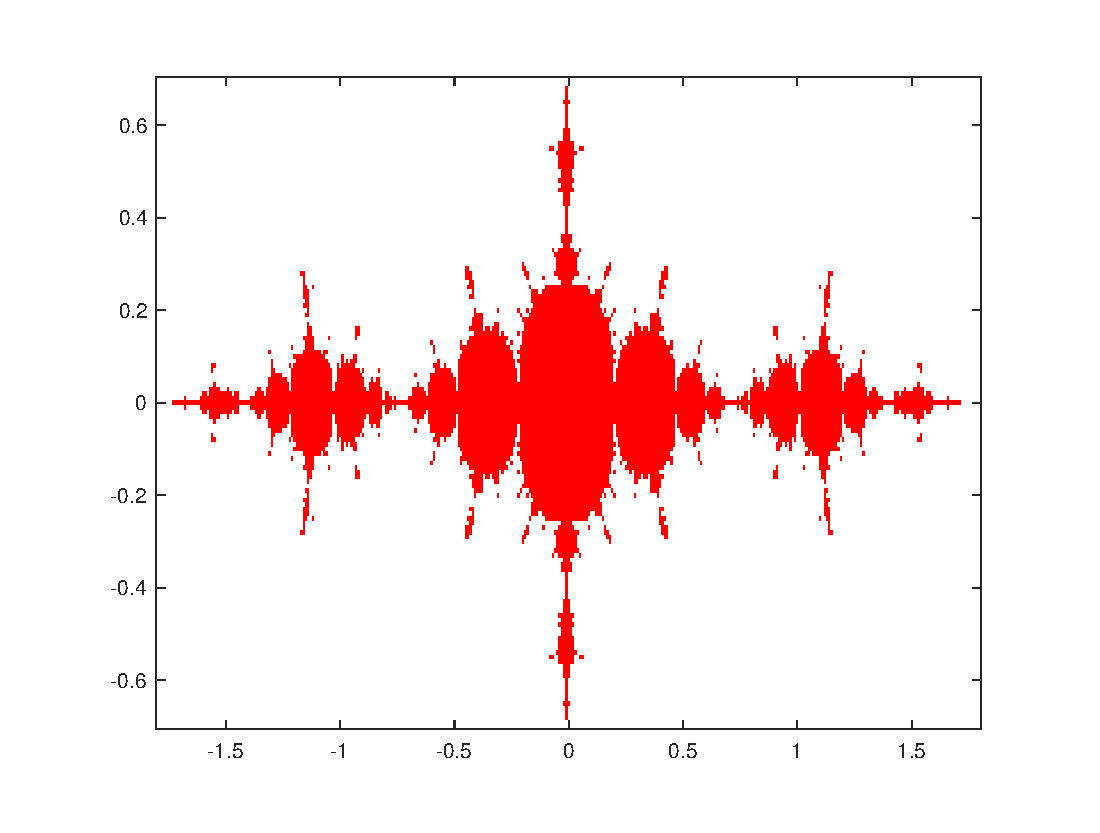
\includegraphics[width=\textwidth]{JuliaSet_fig413.eps}
    \caption{$\phi(z)=z^2-1.25$}
  \end{minipage}
  \hfill
  \begin{minipage}[b]{0.45\textwidth}
    \includegraphics[width=\textwidth]{juliaSet_z2.eps}
    \caption{$\phi(z)=z^2$}
  \end{minipage}
\end{figure}


\section{Generate other examples changing the value of c}
When $|z|> 2$, the iteration method will diverge.\\
The filled Julia sets for different values of c:\\
\begin{figure}[H]
  \centering
  \begin{minipage}[b]{0.45\textwidth}
    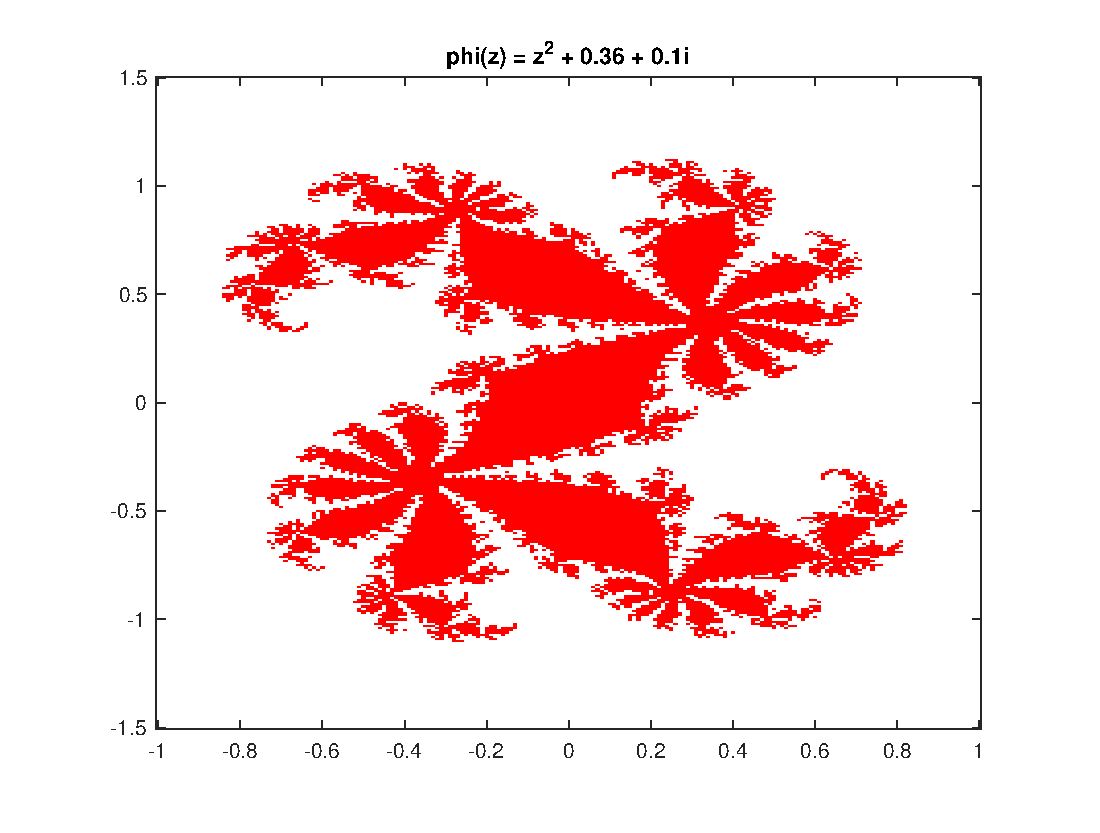
\includegraphics[width=\textwidth]{part2func1.eps}
    \caption{$c = 0.36 + 0.1i$}
  \end{minipage}
  \hfill
  \begin{minipage}[b]{0.45\textwidth}
    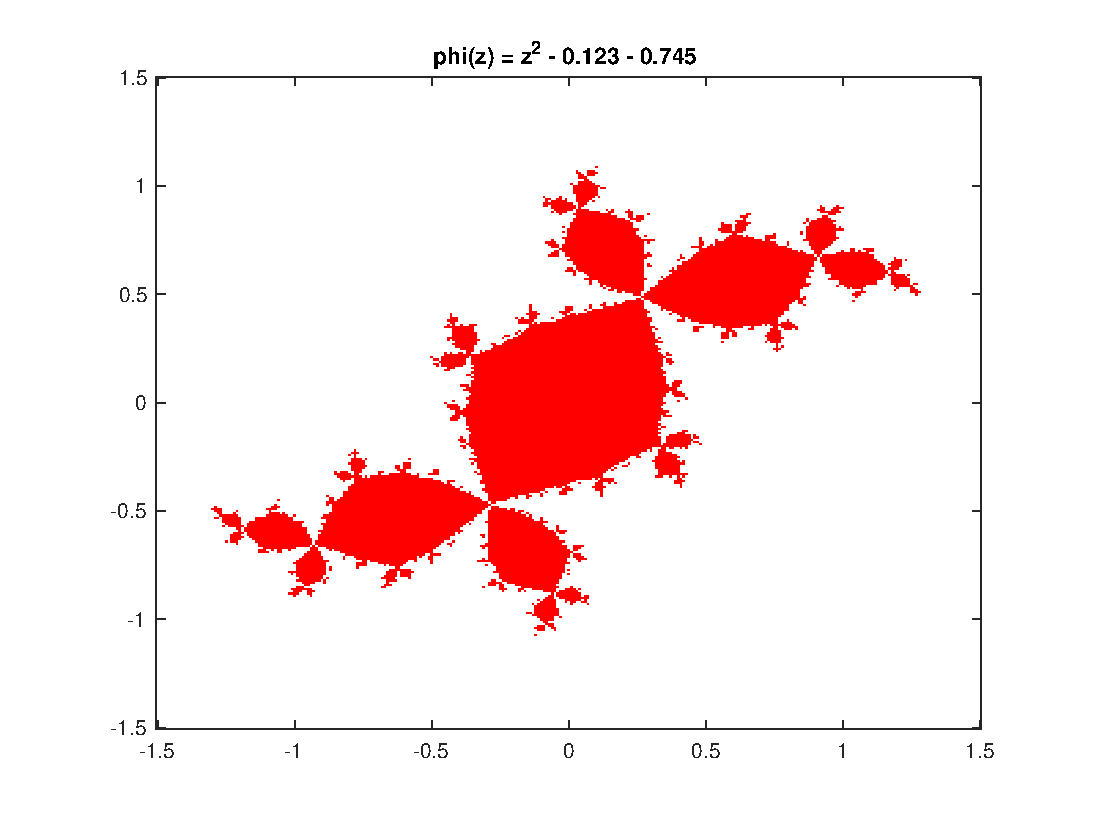
\includegraphics[width=\textwidth]{part2func2.eps}
    \caption{$c = -0.123 - 0.745i$}
  \end{minipage}
   \end{figure}
   
   \begin{figure}[!h]
  \begin{minipage}[b]{0.45\textwidth}
    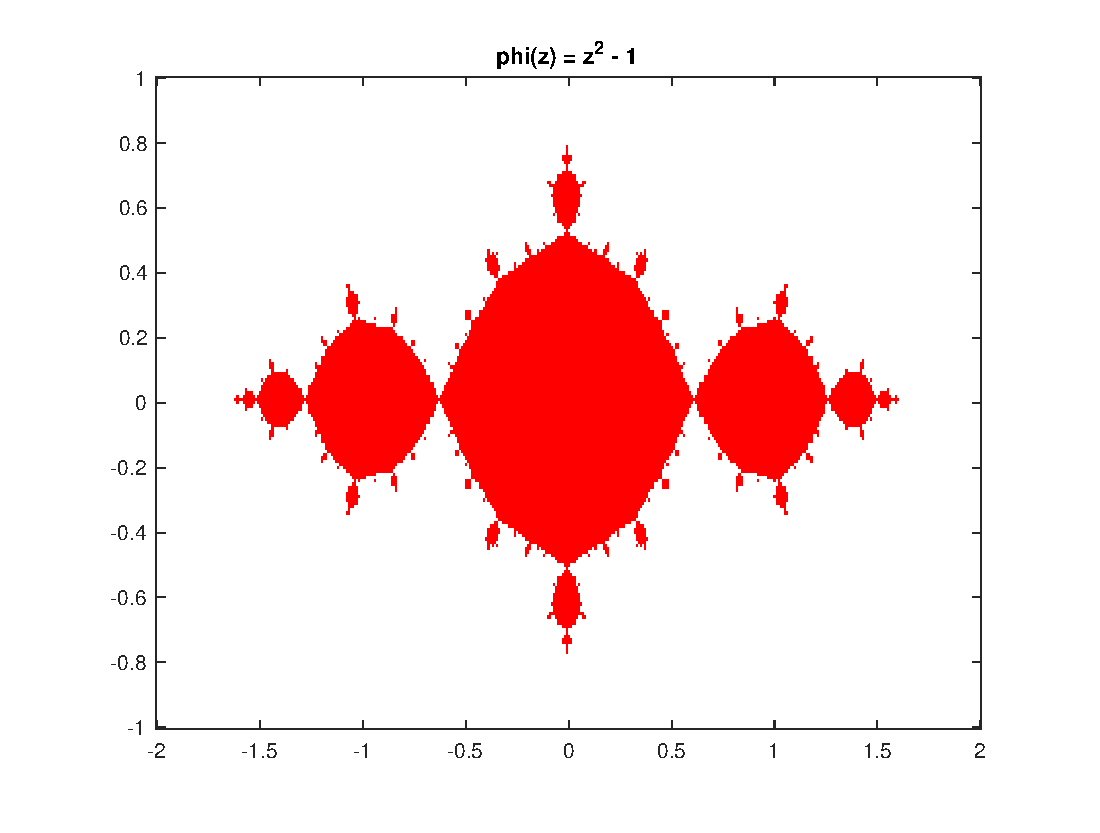
\includegraphics[width=\textwidth]{part2func5.eps}
    \caption{$c = -1$}
  \end{minipage}
  \hfill
  \begin{minipage}[b]{0.45\textwidth}
    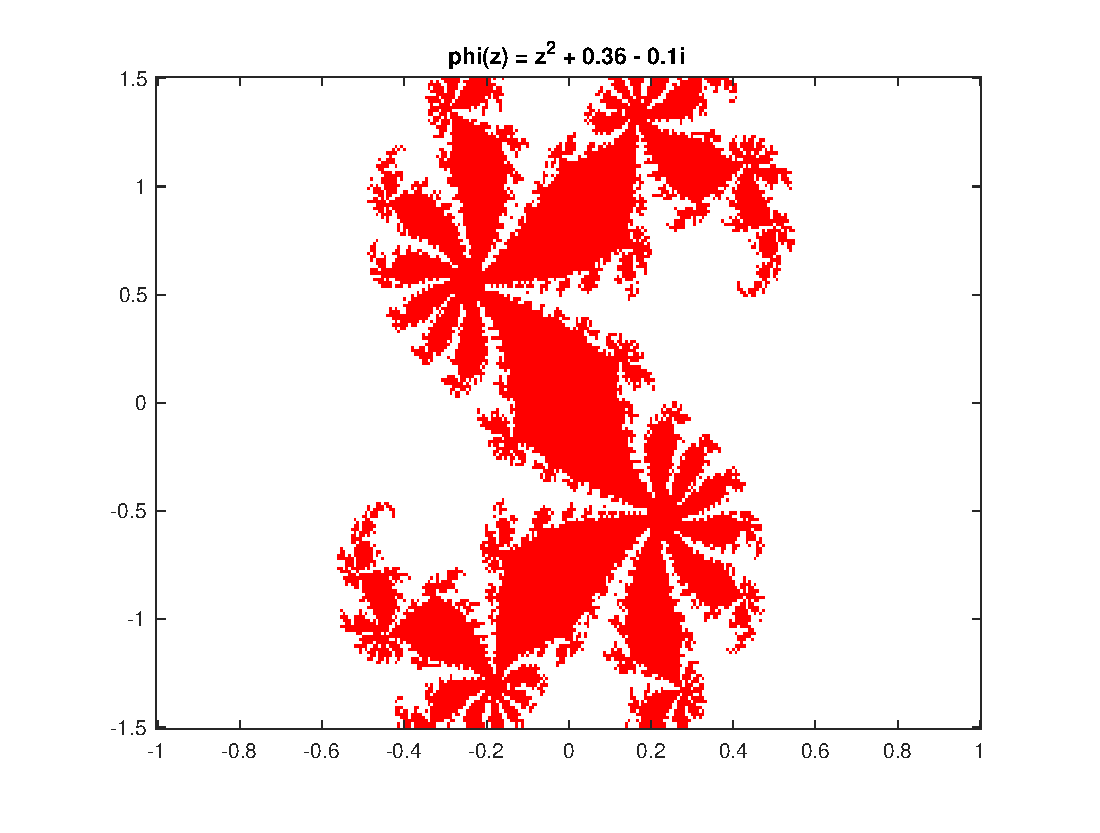
\includegraphics[width=\textwidth]{part2func6.eps}
    \caption{$c = -i$}
  \end{minipage}

\end{figure}

\section{Constructing the Julia Set}
\end{document}  